\clearpage{\pagestyle{empty}\cleardoublepage}

\chapter{Risultati ottenuti}

\begin{flushright}\begin{small}\textit{"Hard science gives sensational results\\ with a horribly boring process."}\\
- Nassim Nicholas Taleb -\\
\end{small}\end{flushright}

Lo sviluppo e la convalida dell'algoritmo sono stati effettuati correggendo immagini in fluorescenza rossa di cellule di fibroblasti, sfruttando apposite immagini di calibrazione di sferette nanometriche, anch'esse fluorescenti nel rosso.

Le immagini di riferimento, utilizzate nella prima e nella seconda fase del programma, sono state acquisite in otto pozzetti di una multiwell: due con sferette ad intensità relativa del 100\% e due del 10\%, due con una mixture di cinque intensità (1\%, 3\%, 10\%, 30\% e 100\%) ed infine nelle rimanenti è stato posto unicamente il mezzo di coltura, così da studiare la fluorescenza di background indotta dalla sorgente.
Il riempimento di ogni pozzetto ha previsto l'agitazione sia manuale che con sonificatore delle sferette e l'iniezione con le pipette ghilson di $220\ \mu l$ di terreno completo e delle sferette di calibrazione: $10\ \mu l$ per i quattro pozzetti ad intensità unica e $2\ \mu l$ per i due pozzetti a cinque intensità.
Tuttavia una delle due immagini con sferette aventi differente luminosità ha mostrato un'errata composizione del campione e perciò è stata rimossa in fase di elaborazione e testing.

L'analisi che segue esamina l'efficacia dell'algoritmo nella rimozione della disomogeneità poiché, come visto in precedenza, il difetto della fluorescenza di sfondo viene semplicemente eliminato sottraendo il parametro costante identificato nella seconda fase.

Tale capitolo si propone di esporre e commentare i risultati conseguiti dall'algoritmo tramite due analisi: 
\begin{itemize}
 \item gli istogrammi dell'intensità dell'immagine
 \item la dipendenza dell'intensità dalla distanza dal centro
\end{itemize}

Queste due rielaborazioni verranno affrontate sulla base di grafici e risultati ottenuti applicando l'algoritmo sull'immagine dei fibroblasti, nel particolar caso in cui la prima immagine di calibrazione sia costituita da un campione di sferette con intensità relativa del 10\%.
Successivamente, per poter avere una miglior valutazione dell'efficacia del programma, verrà eseguito un confronto tra i risultati ottenuti utilizzando nella prima fase dell'algoritmo quattro distinte immagini di calibrazione, acquisite col microscopio a fluorescenza.

In Appendice B mostriamo le immagini per dare un esempio qualitativo del risultato della correzione.

\section{Distribuzione delle intensità}

Come visto, la disomogeneità di illuminazione comporta la rilevazione di immagini con intensità maggiore al centro rispetto al margine (a parità di densità di fluorocromo), comportando di conseguenza un'alterazione della distribuzione delle intensità. 
Tale fenomeno viene attenuato in modo sostanziale tramite l'azione della prima fase dell'algoritmo, la quale agisce proprio sul difetto preso in considerazione.

Il cambiamento della distribuzione di intensità provocato dal software è percepibile graficando gli istogrammi relativi alle varie intensità rilevate all'interno dell'immagine in fase pre e post correzione.
L'istogramma osservato nell'immagine non corretta è molto ampio, in quanto alla normale incertezza nel valore della fluorescenza delle sferette si aggiunge un bias legato alla loro posizione spaziale.
In seguito alla correzione ci aspettiamo un istogramma approssimativamente gaussiano con un'incertezza minore, in quanto la componente spaziale dovrebbe essere stata corretta.

In \figurename~\ref{fig:isto1} si vede l'istogramma delle intensità delle nanosfere della prima immagine di calibrazione.
È chiaramente visibile una riduzione dell'incertezza, con un picco secondario approssimativamente localizzato al doppio dell'intensità del picco primario, corrispondente alle sfere sovrapposte (dettaglio non presente nel precedente istogramma in quanto indistinguibile per via dell'ampiezza della distribuzione).
Tale risultato è proprio ciò a cui si mirava, dato che le sferette contenute nel campione risultano avere la medesima intensità.

In \figurename~\ref{fig:isto2} si vede l'istogramma logaritmico delle intensità delle nanosfere a 5 intensità. 
È chiaro il miglioramento nella qualità dell'istogramma, in cui dopo la correzione i 5 picchi sono chiaramente distinti e di ampiezza confrontabile.

In \figurename~\ref{fig:isto3} abbiamo l'istogramma dei massimi di intensità di fluorescenza delle cellule, prima e dopo la correzione.
In questo caso il miglioramento è meno visibile in quanto alle incertezze strumentali si sovrappongono quelle di natura biologica.
Per tale motivo le intensità rilevate nell'immagine è giusto che si estendano entro un range abbastanza ampio, proprio perché a seconda della concentrazione delle probes fluorescenti nella cellula sarà differente il grado di luminosità sviluppato.

\begin{figure}
 \centering
 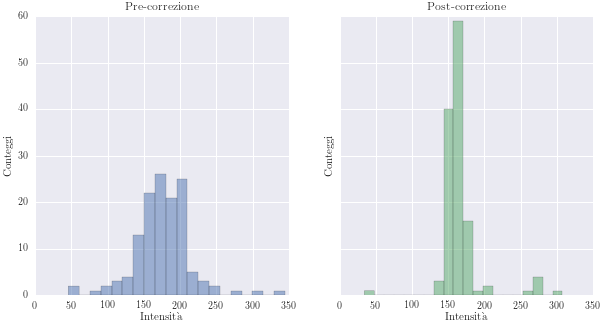
\includegraphics[scale=.55]{img/CAP4isto1.png}
 \caption{\small{Istogrammi relativi alle intensità dei massimi della prima immagine di calibrazione, costituita da sferette con stessa intensità. Il grafico a sinistra è associato alla fase di pre-correzione (\figurename~\ref{fig:unaint}), mentre quello a destra alla fase di post-correzione (\figurename~\ref{fig:unaintcorr}). Come previsto, l'algoritmo di correzione fa sì che le intensità risultino molto più piccate attorno un unico valore.}}
 \label{fig:isto1}
\end{figure}

\begin{figure}
 \centering
 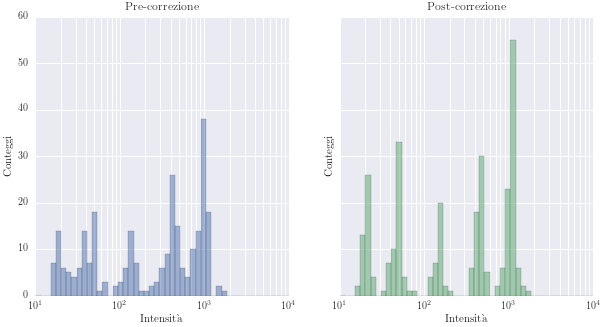
\includegraphics[scale=.55]{img/CAP4isto2.png}
 \caption{\small{Istogrammi relativi alle intensità dei massimi della seconda immagine di calibrazione, costituita da sferette con cinque intensità differenti. Il grafico a sinistra è associato alla fase di pre-correzione (\figurename~\ref{fig:piuint}), mentre quello a destra alla fase di post-correzione (\figurename~\ref{fig:piuintcorr}). Come previsto, l'algoritmo di correzione fa sì che le intensità risultino molto più piccate attorno ai cinque valori medi delle gaussiane, rendendo queste molto più definite.}}
 \label{fig:isto2}
\end{figure}

\begin{figure}
 \centering
 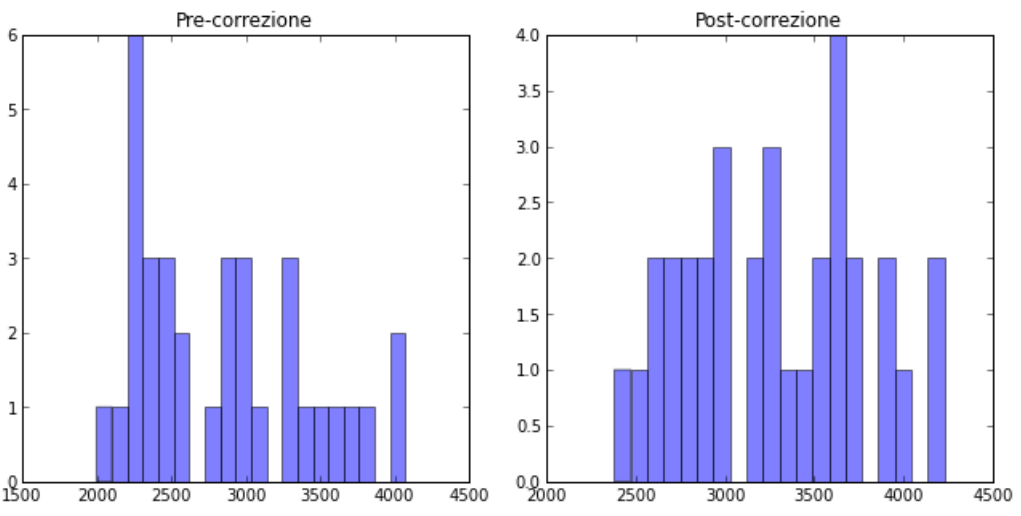
\includegraphics[scale=.55]{img/CAP4isto3.png}
 \caption{\small{Istogrammi relativi alle intensità dei massimi dell'immagine delle cellule di fibroblasti. Il grafico a sinistra è associato alla fase di pre-correzione (\figurename~\ref{fig:cell}), mentre quello a destra alla fase di post-correzione (\figurename~\ref{fig:cellcorr}). Come previsto, l'algoritmo di correzione determina una miglior simmetria della distribuzione di intensità.}}
 \label{fig:isto3}
\end{figure}


\section{Dipendenza spaziale dell'intensità}

In statistica, data un'ipotesi nulla ($H_0$), questa la si può accettare o rifiutare sulla base del cosiddetto \textit{p-value}, parametro probabilistico con valore compreso tra 0 ed 1.
Esso può essere definito come livello di significatività assegnato e quantifica la ``forza dell'evidenza'' contro l'ipotesi nulla $H_0$, a favore dell'alternativa, espressa dai dati osservati su un determinato campione. 
Per esempio, assegnato un valore di soglia, se il p-value è maggiore di tale valore allora $H_0$ non viene rigettata, in caso contrario sì.
Di conseguenza il p-value esprime quanto sia plausibile che i dati osservati si ottengano essendo vera l’ipotesi nulla: un p-value grande esprime evidenza sperimentale a favore dell'ipotesi nulla, mentre un suo valore piccolo un'evidenza a favore dell'ipotesi alternativa.\todo{rivedere queste definizioni, non sono corrette}

Come precedentemente osservato, la presenza di disomogenea di illuminazione comporta una dipendenza dell'intensità dei pixel (a parità di densità di fluoroforo) dalla loro posizione.
In modo compatibile con la nostra ipotesi di lavoro stimiamo questa dipendenza come funzione della sola distanza dal centro dell'immagine.
Questa relazione non è lineare, ma è possibile calcolare il p-value di questa dipendenza approssimandolo come tale.
Il p-value rapprenta quindi la probabilità di osservare l'andamento sperimentale sotto l'ipotesi nulla che non ci sia alcuna dipendenza.

A tal proposito è stata valutata per ogni punto di massimo dell'immagine (centro delle sferette per le immagini di calibrazione e nuclei delle cellule per l'immagine da correggere) la distanza dall'origine, intesa come punto centrale dell'immagine stessa.
Le immagini sono state quindi ridotte ad una serie di coppie intensità-distanza radiale.
Per ottenere il valore del p-value si è quindi sfruttata la funzione \textit{linregress}, in grado di valutare la relazione lineare esistente o meno tra le intensità dei punti di massimo e le distanze radiali associate.
Tale funzione restituisce il p-value come semplice parametro di return e questo viene valutato prendendo come ipotesi nulla $H_0$ il fatto che la slope sia nulla, quindi maggiore sarà il p-value e più plausibile sarà assumere l'assenza di una dipendenza spaziale dell'intensità.

\begin{figure}
 \centering
 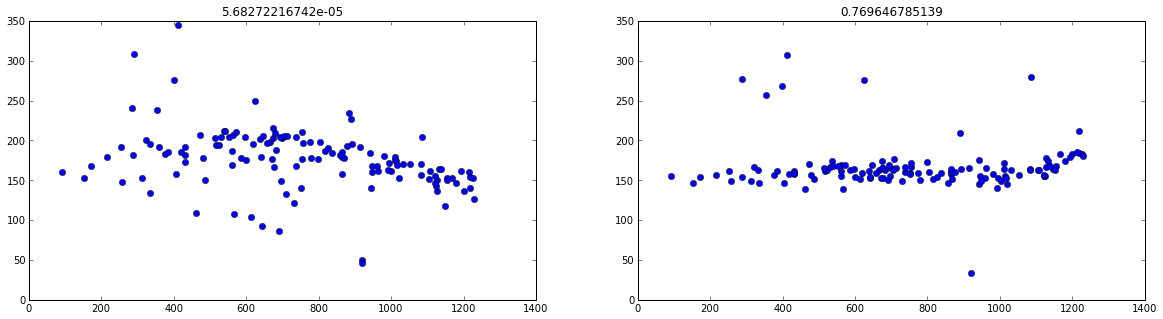
\includegraphics[scale=.55]{img/CAP4pvalue1.png}
 \caption{\small{Distribuzione delle intensità dei massimi in funzione della distanza radiale, relativa alla prima immagine di calibrazione. Il grafico in alto è associato alla fase di pre-correzione (\figurename~\ref{fig:unaint}), mentre quello in basso alla fase di post-correzione (\figurename~\ref{fig:unaintcorr}). Al di sopra sono riportati i valori del p-value associato alla corrispondente regressione lineare. Come previsto, il p-value si avvicina ad 1 una volta applicato l'algoritmo sull'immagine.}}
 \label{fig:pvalue1}
\end{figure}

\begin{figure}
 \centering
 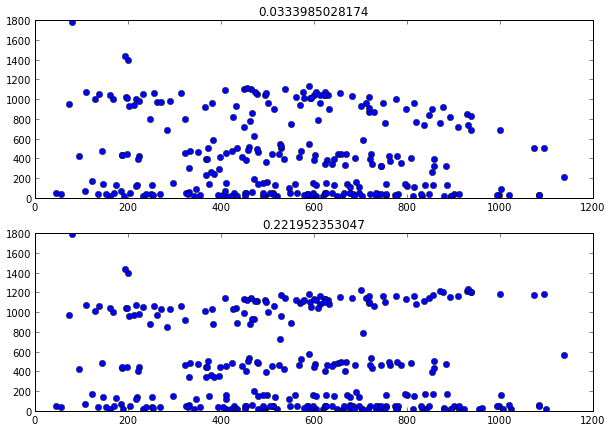
\includegraphics[scale=.55]{img/CAP4pvalue2.png}
 \caption{\small{Distribuzione delle intensità dei massimi in funzione della distanza radiale, relativa alla seconda immagine di calibrazione. Il grafico in alto è associato alla fase di pre-correzione (\figurename~\ref{fig:piuint}), mentre quello in basso alla fase di post-correzione (\figurename~\ref{fig:piuintcorr}). Al di sopra sono riportati i valori del p-value associato alla corrispondente regressione lineare. Come previsto, il p-value si avvicina ad 1 una volta applicato l'algoritmo sull'immagine.}}
 \label{fig:pvalue2}
\end{figure}

\begin{figure}
 \centering
 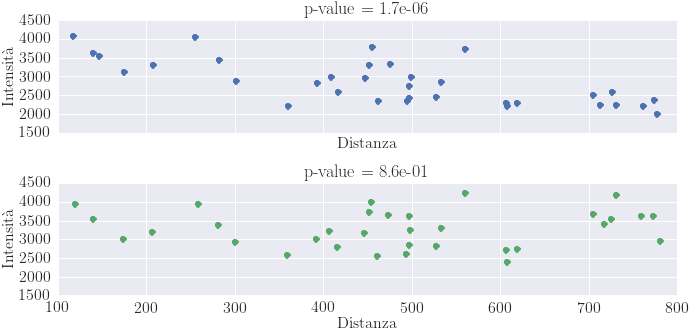
\includegraphics[scale=.55]{img/CAP4pvalue3.png}
 \caption{\small{
 Distribuzione delle intensità dei massimi in funzione della distanza radiale, relativa all'immagine delle cellule di fibroblasti. Il grafico in alto è associato alla fase di pre-correzione (\figurename~\ref{fig:cell}), mentre quello in basso alla fase di post-correzione (\figurename~\ref{fig:cellcorr}). Al di sopra sono riportati i valori del p-value associato alla corrispondente regressione lineare. Come previsto, il p-value si avvicina ad 1 una volta applicato l'algoritmo sull'immagine.}}
 \label{fig:pvalue3}
\end{figure}

Come si evince dalle Figure \ref{fig:pvalue1}, \ref{fig:pvalue2}, \ref{fig:pvalue3}, il p-value della relazione parte da valori molto bassi, che risultano significativi usando le comuni soglie di significatività.
Dopo la correzione questi risultano più elevati, compatibili con la distribuzione uniforme che ci si attende dalla distribuzione nulla.
Questo implica che dopo la correzione i dati sono compatibili con l'assenza di correlazione, sia nelle immagini di calibrazione che nell'immagine dei fibroblasti. 
Perciò, sulla base di tale analisi, dopo aver corretto l'immagine la dipendenza spaziale dell'intensità, inizialmente presente a causa della disomogeneità dell'illuminazione creata dalla sorgente, può essere considerata sostanzialmente non significativa.


\section{Confronto tra differenti immagini di calibrazione}

Come detto in precedenza, tale algoritmo permette la correzione dell'immagine a fluorescenza sulla base di due ulteriori immagini: la prima deve avere sferette di calibrazione a stessa intensità e viene sfruttata per la correzione della disomogeneità di illuminazione, mentre la seconda deve contenere sferette con differenti luminosità ed è necessaria per la rimozione del parametro di background. 
\'E sulla base di queste due ultime immagini che si ottengono i parametri necessari per la correzione di quella in esame.
Per tale motivo sono stati confrontati i risultati ottenuti con quattro distinte immagini di calibrazione ad una sola intensità: due con intensità relativa del 10\% (chiamate successivamente $10\%_1$ e $10\%_2$) e due con intensità relativa del 100\% (chiamate successivamente $100\%_1$ e $100\%_2$).

Dalle Figure \ref{fig:gauss1}, \ref{fig:gauss2}, \ref{fig:gauss3} e \ref{fig:gauss4} è evidente il fatto che differenti immagini di calibrazioni comportino differenti superfici tridimensionali risultanti dal fit di maximum likelihood, indipendentemente dall'intensità relativa delle sferette.

\begin{figure}
 \centering
 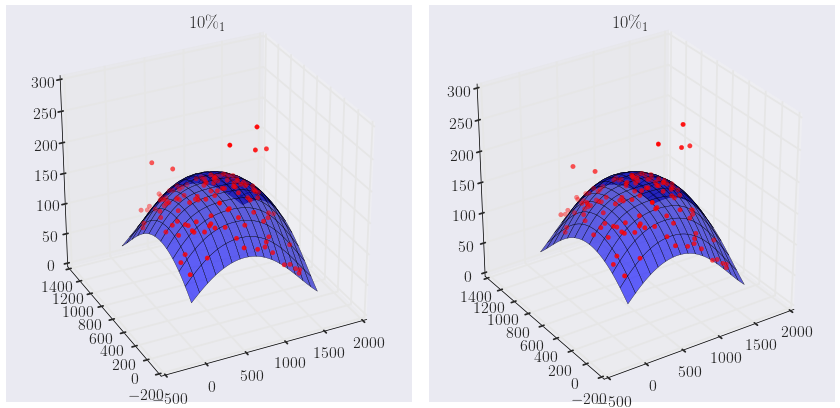
\includegraphics[scale=.45]{img/CAP4gauss1.png}
 \caption{\small{Immagine in visione ``cross eyed stereoscopic'' corrispondente alla prima immagine di calibrazione con intensità relativa del 10\%: i puntini rappresentano i massimi mentre la superficie è quella risultante dal fit di maximum likelihood.}}
 \label{fig:gauss1}
\end{figure}

\begin{figure}
 \centering
 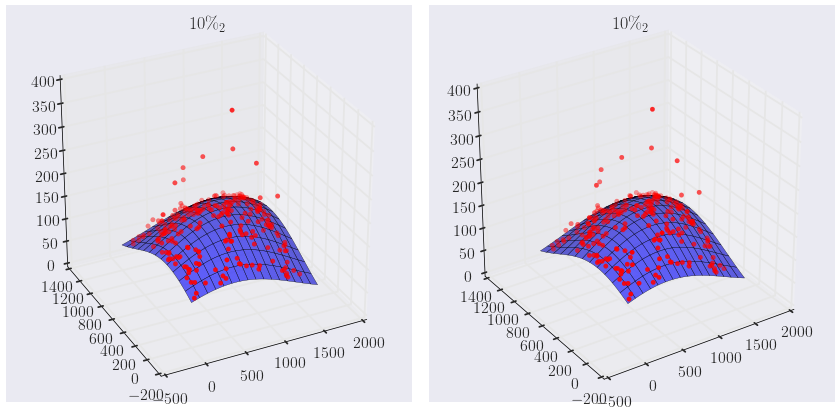
\includegraphics[scale=.45]{img/CAP4gauss2.png}
 \caption{\small{Immagine in visione ``cross eyed stereoscopic'' corrispondente alla seconda immagine di calibrazione con intensità relativa del 10\%: i puntini rappresentano i massimi mentre la superficie è quella risultante dal fit di maximum likelihood.}}
 \label{fig:gauss2}
\end{figure}

\begin{figure}
 \centering
 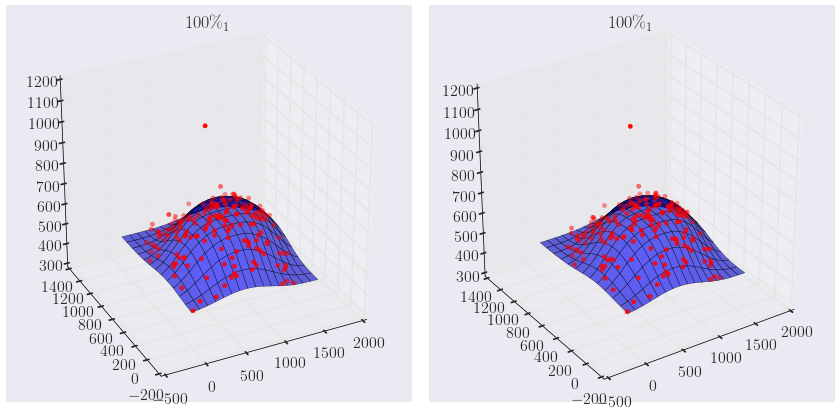
\includegraphics[scale=.45]{img/CAP4gauss3.png}
 \caption{\small{Immagine in visione ``cross eyed stereoscopic'' corrispondente alla prima immagine di calibrazione con intensità relativa del 100\%: i puntini rappresentano i massimi mentre la superficie è quella risultante dal fit di maximum likelihood.}}
 \label{fig:gauss3}
\end{figure}

\begin{figure}
 \centering
 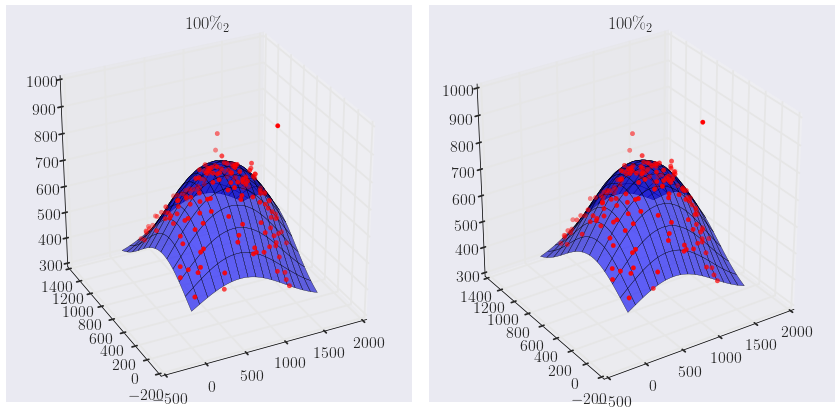
\includegraphics[scale=.45]{img/CAP4gauss4.png}
 \caption{\small{Immagine in visione ``cross eyed stereoscopic'' corrispondente alla seconda immagine di calibrazione con intensità relativa del 100\%: i puntini rappresentano i massimi mentre la superficie è quella risultante dal fit di maximum likelihood.}}
 \label{fig:gauss4}
\end{figure}

Per poter avere un'analisi di carattere più quantitativo sono stati visualizzati i parametri $bg,\ maxint,\ cx,\ cy,\ dsx,\ dsy,\ corr$ ed $e$ ottenuti dalla stima di massima verosimiglianza (capitolo 3.1) eseguita nei quattro casi (Figure \ref{fig:cx}, \ref{fig:cy}, \ref{fig:dsx}, \ref{fig:dsy} \ref{fig:bg}, \ref{fig:intmax}, \ref{fig:corr} e \ref{fig:e}).
Queste stime di massima verosimiglianza sono state inoltre raccolte nella \tablename~\ref{TABris}, assieme al primo parametro approssimato di background $bg_0$, calcolato inizialmente come massimo delle mode di ogni riga della matrice bidimensionale corrispondente all'immagine.

Dall'analisi di questi risultati si nota che differenti immagini di calibrazione comportano in genere differenti parametri, sebbene i valori si mantengano solitamente entro lo stesso ordine di grandezza. 
Per tale motivo si può affermare che la nostra procedura di calibrazione sembra dare una risposta coerente fra diverse immagini di calibrazione.
Tuttavia per avere una miglior valutazione dell'effetto che tali differenze potrebbero comportare sulla correzione finale dell'immagine bisognerebbe eseguire elaborazioni successive, più raffinate rispetto alla semplice analisi qui riportata.

Nelle Figure \ref{fig:c1}, \ref{fig:c2}, \ref{fig:c3}, \ref{fig:c4} sono riportate le matrici di correlazione tra le stime dei parametri per le quattro differenti immagini di calibrazione.

\begin{table}
 \begin{center}
\begin{small}
\begin{tabular}{lcccc}
\hline\hline
&$\mathbf{10\%_1}$&$\mathbf{10\%_2}$&$\mathbf{100\%_1}$&$\mathbf{100\%_2}$\\
\hline
$\mathbf{bg_0}$& 19 & 19 & 13 & 13\\
\hline
$\mathbf{cx}$&$767\pm11$&$832\pm10$&$881\pm9$&$831\pm10$\\
$\mathbf{cy}$&$587\pm9$&$583\pm7$&$583\pm6 $&$608\pm6$\\
$\mathbf{dsx}$&$823\pm205$&$ 797\pm131$&$568 \pm17$&$663\pm66$\\
$\mathbf{dsy}$&$646\pm159$&$524\pm85$&$ 409\pm11$&$453\pm44$\\
$\mathbf{corr}$&$-0.29\pm0.06$&$-0.65\pm0.05 $&$-0.51\pm0.05$&$-0.49\pm0.05$\\
$\mathbf{bg}$&$1.58\cdot 10^{-6}\pm102$&$23\pm40 $&$452\pm13$&$341\pm82$\\
$\mathbf{maxint}$&$167\pm104$&$150\pm41$&$229\pm15$&$414\pm87$\\
$\mathbf{e}$&$3.2\pm0.6$&$2.1\pm0.3$&$3.6\pm0.4$&$2.5\pm0.4$\\
\hline\hline
\end{tabular}
\caption{\small{Confronto dei parametri ottenuti nella prima fase dell'algoritmo con quattro distinte immagini di calibrazione ad una sola intensità. Per ciascun parametro del fit vengono riportate la miglior stima e la deviazione standard associata, ottenute dalla procedura di fit. La precisione dei valori risulta elevata proprio poiché non si tratta di incertezze associate alla stima, bensì dei valori che approssimano localmente la funzione di likelihood con una distribuzione gaussiana.}}
\label{TABris}
\end{small}
\end{center}
\end{table}

\begin{figure}
 \centering
 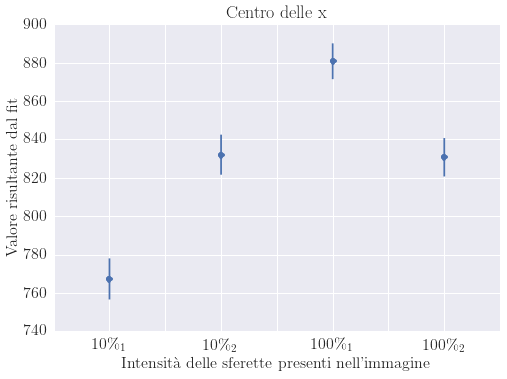
\includegraphics[scale=.50]{img/CAP4cx.png}
 \caption{\small{Parametro $cx$ (centro delle x) e intervallo di confidenza al 95\%, ottenuti tramite il fit di maximum likelihood presente nell'algoritmo, per le quattro differenti immagini di calibrazione ad una sola intensità.}}
 \label{fig:cx}
\end{figure}

\begin{figure}
 \centering
 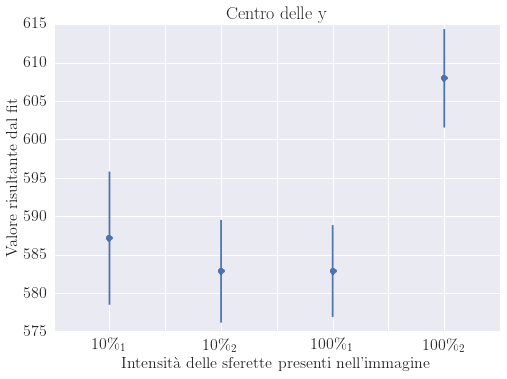
\includegraphics[scale=.50]{img/CAP4cy.png}
 \caption{\small{Parametro $cy$ (centro delle y) e intervallo di confidenza al 95\%, ottenuti tramite il fit di maximum likelihood presente nell'algoritmo, per le quattro differenti immagini di calibrazione ad una sola intensità.}}
 \label{fig:cy}
\end{figure}

\begin{figure}
 \centering
 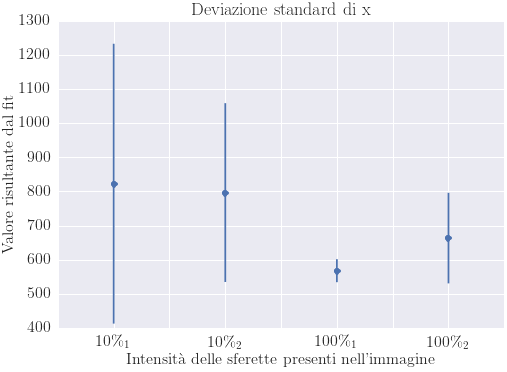
\includegraphics[scale=.50]{img/CAP4dsx.png}
 \caption{\small{Parametro $dsx$ (deviazione standard di x) e intervallo di confidenza al 95\%, ottenuti tramite il fit di maximum likelihood presente nell'algoritmo, per le quattro differenti immagini di calibrazione ad una sola intensità.}}
 \label{fig:dsx}
\end{figure}

\begin{figure}
 \centering
 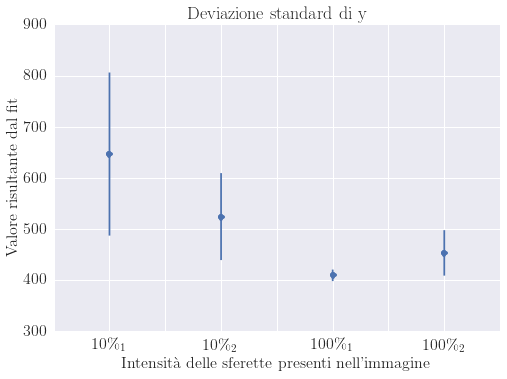
\includegraphics[scale=.50]{img/CAP4dsy.png}
 \caption{\small{Parametro $dsy$ (deviazione standard di y) e intervallo di confidenza al 95\%, ottenuti tramite il fit di maximum likelihood presente nell'algoritmo, per le quattro differenti immagini di calibrazione ad una sola intensità.}}
 \label{fig:dsy}
\end{figure}

\begin{figure}
 \centering
 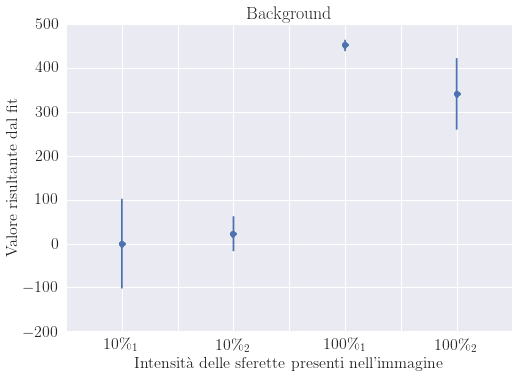
\includegraphics[scale=.50]{img/CAP4bg.png}
 \caption{\small{Parametro $bg$ (background) e intervallo di confidenza al 95\%, ottenuti tramite il fit di maximum likelihood presente nell'algoritmo, per le quattro differenti immagini di calibrazione ad una sola intensità.}}
 \label{fig:bg}
\end{figure}

\begin{figure}
 \centering
 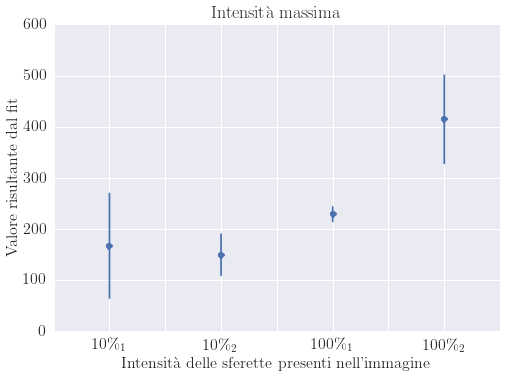
\includegraphics[scale=.50]{img/CAP4intmax.png}
 \caption{\small{Parametro $maxint$ (intensità massima) e intervallo di confidenza al 95\%, ottenuti tramite il fit di maximum likelihood presente nell'algoritmo, per le quattro differenti immagini di calibrazione ad una sola intensità.}}
 \label{fig:intmax}
\end{figure}

\begin{figure}
 \centering
 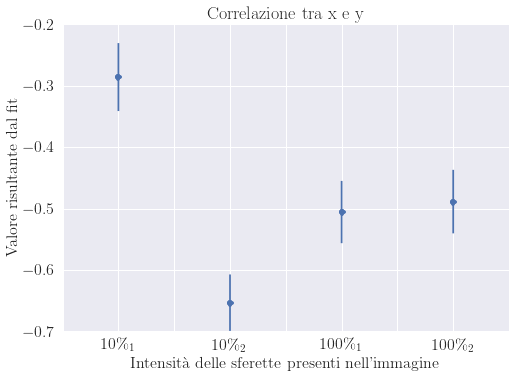
\includegraphics[scale=.50]{img/CAP4corr.png}
 \caption{\small{Parametro $corr$ (correlazione tra x ed y) e intervallo di confidenza al 95\%, ottenuti tramite il fit di maximum likelihood presente nell'algoritmo, per le quattro differenti immagini di calibrazione ad una sola intensità.}}
 \label{fig:corr}
\end{figure}

\begin{figure}
 \centering
 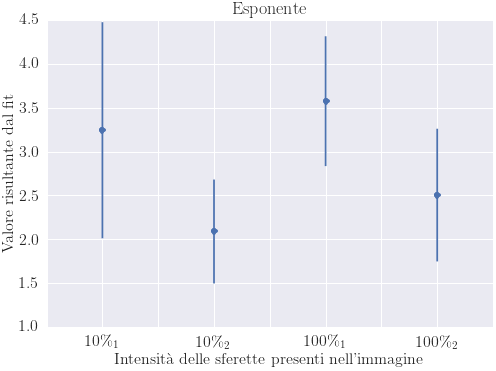
\includegraphics[scale=.50]{img/CAP4e.png}
 \caption{\small{Parametro $e$ (esponente) e intervallo di confidenza al 95\%, ottenuti tramite il fit di maximum likelihood presente nell'algoritmo, per le quattro differenti immagini di calibrazione ad una sola intensità.}}
 \label{fig:e}
\end{figure}

\begin{figure}
 \centering
 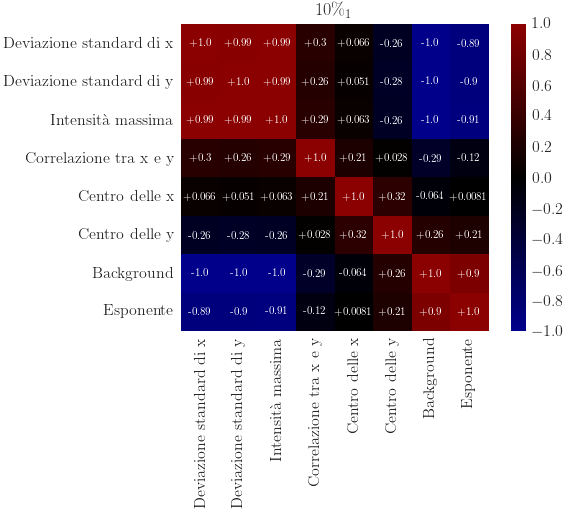
\includegraphics[scale=.48]{img/CAP4c1.png}
 \caption{\small{Matrice di correlazione tra le stime dei parametri ottenuti dal fit di maximum likelihood per l'immagine di calibrazione $10\%_1$.}}
 \label{fig:c1}
\end{figure}

\begin{figure}
 \centering
 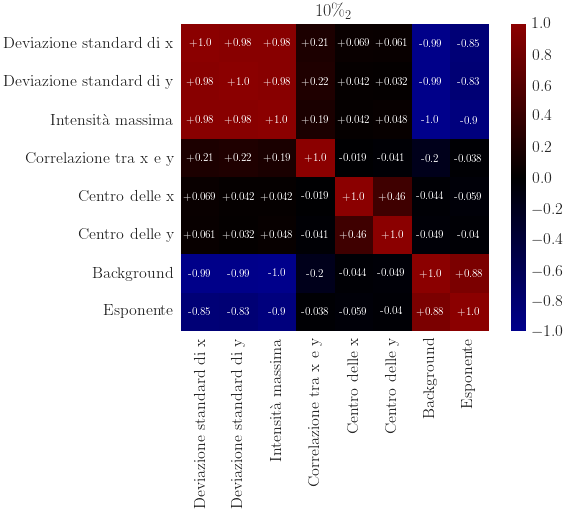
\includegraphics[scale=.48]{img/CAP4c2.png}
 \caption{\small{Matrice di correlazione tra le stime dei parametri ottenuti dal fit di maximum likelihood per l'immagine di calibrazione $10\%_2$.}}
 \label{fig:c2}
\end{figure}

\begin{figure}
 \centering
 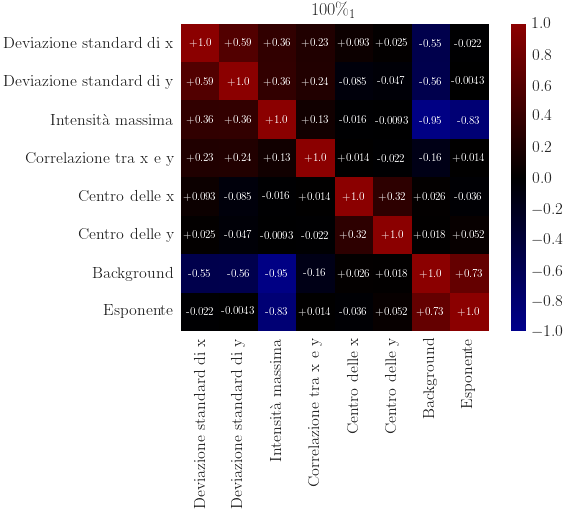
\includegraphics[scale=.48]{img/CAP4c3.png}
 \caption{\small{Matrice di correlazione tra le stime dei parametri ottenuti dal fit di maximum likelihood per l'immagine di calibrazione $100\%_1$.}}
 \label{fig:c3}
\end{figure}

\begin{figure}
 \centering
 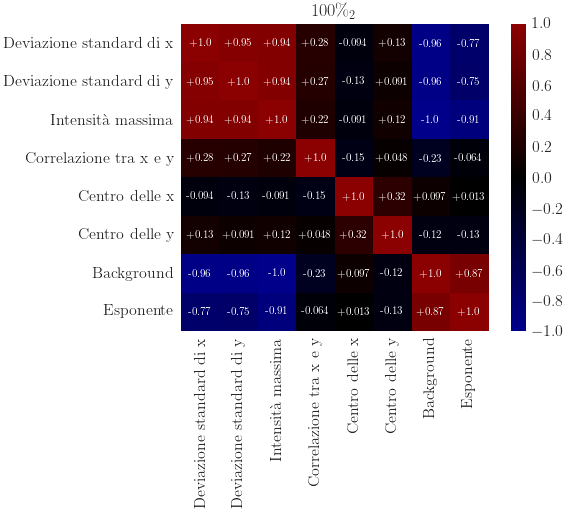
\includegraphics[scale=.48]{img/CAP4c4.png}
 \caption{\small{Matrice di correlazione tra le stime dei parametri ottenuti dal fit di maximum likelihood per l'immagine di calibrazione $100\%_2$.}}
 \label{fig:c4}
\end{figure}


